\section{ First section}


Some text

A list:


1.   first case;
2.   second case.

A bold text, *an italic text*, a code text, a normal text.

\subsection{# Subsection with code}


There is a simple code above.

\begin{lstlisting}[language={Python},caption={}]
print("Hello world")
\end{lstlisting}


\begin{lstlisting}[language={},caption={Результат выполнения программы}]
Hello world

\end{lstlisting}

\section{ Table section}


There is a code that generetes a table as output.

\begin{lstlisting}[language={Python},caption={}]
import pandas as pd

data = [
    ["Gleb", "Programmer", 20],
    ["Xkentiy", "3D", 21],
    ["Nikita", "Sience", 2023]
]

table = pd.DataFrame(data=data, index=[i for i in range(1, 3+1)], columns=["Name", "Job", "Age"])

table
\end{lstlisting}


\begin{table}[h!]
    \centering
    \caption{}
    \begin{tabular}{|c|c|c|}
    \hline
Name & Job & Age \\ \hline
Gleb & Programmer & 20 \\
Xkentiy & 3D & 21 \\
Nikita & Sience & 2023 \\

	\hline
    \end{tabular}
    \label{tab:my\_label}
\end{table}
\section{ Plot section}


There is a code that generate an image as output.



\begin{lstlisting}[language={Python},caption={}]
import matplotlib.pyplot as plt

def f(x):
  return x * x

X = [i / 5 for i in range(0, 50)]
Y = [f(x) for x in X]

plt.plot(X, Y)
plt.show()
\end{lstlisting}


\begin{figure}[h!]
  \centering
  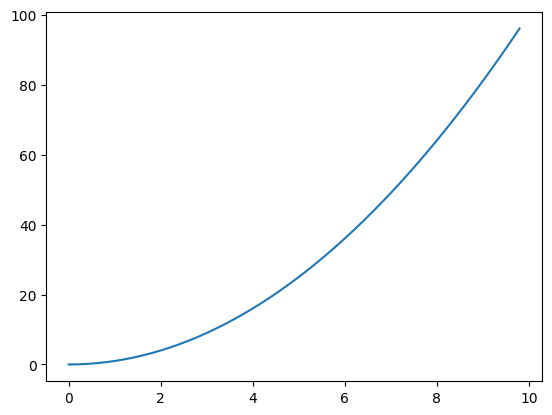
\includegraphics[width=0.9\textwidth]{img/1.png}
  \caption{}
  \label{fig:1}
\end{figure}


